\section{Learning Diffusion Schr\"odinger Bridges from Sparse Trajectories} \label{sec:sb_align}

% TODO: Update with camera-ready version.
\looseness -1 \emph{Interpolation}, the task of transforming one given distribution into another, lies at the heart of many modern machine learning applications such as single-cell genomics \citep{tong2020trajectorynet, schiebinger2019optimal, bunne2022supervised}, meteorology \citep{fisher2009data}, and robotics \citep{chen2021optimal}. To this end, \acrlongpl{DSB} \citep{de2021diffusion,chen2021likelihood,vargas2021solving,liu2022deep} have recently emerged as a powerful paradigm due to their ability to generalize prior deep diffusion-based models, notably \acrlong{SMLD}
\citep{song2019generative,song2020score} and \acrlongpl{DDPM} \citep{ho2020denoising}, which have achieved the state-of-the-art on many generative modeling problems.

\begin{figure}[t]
    \centering
    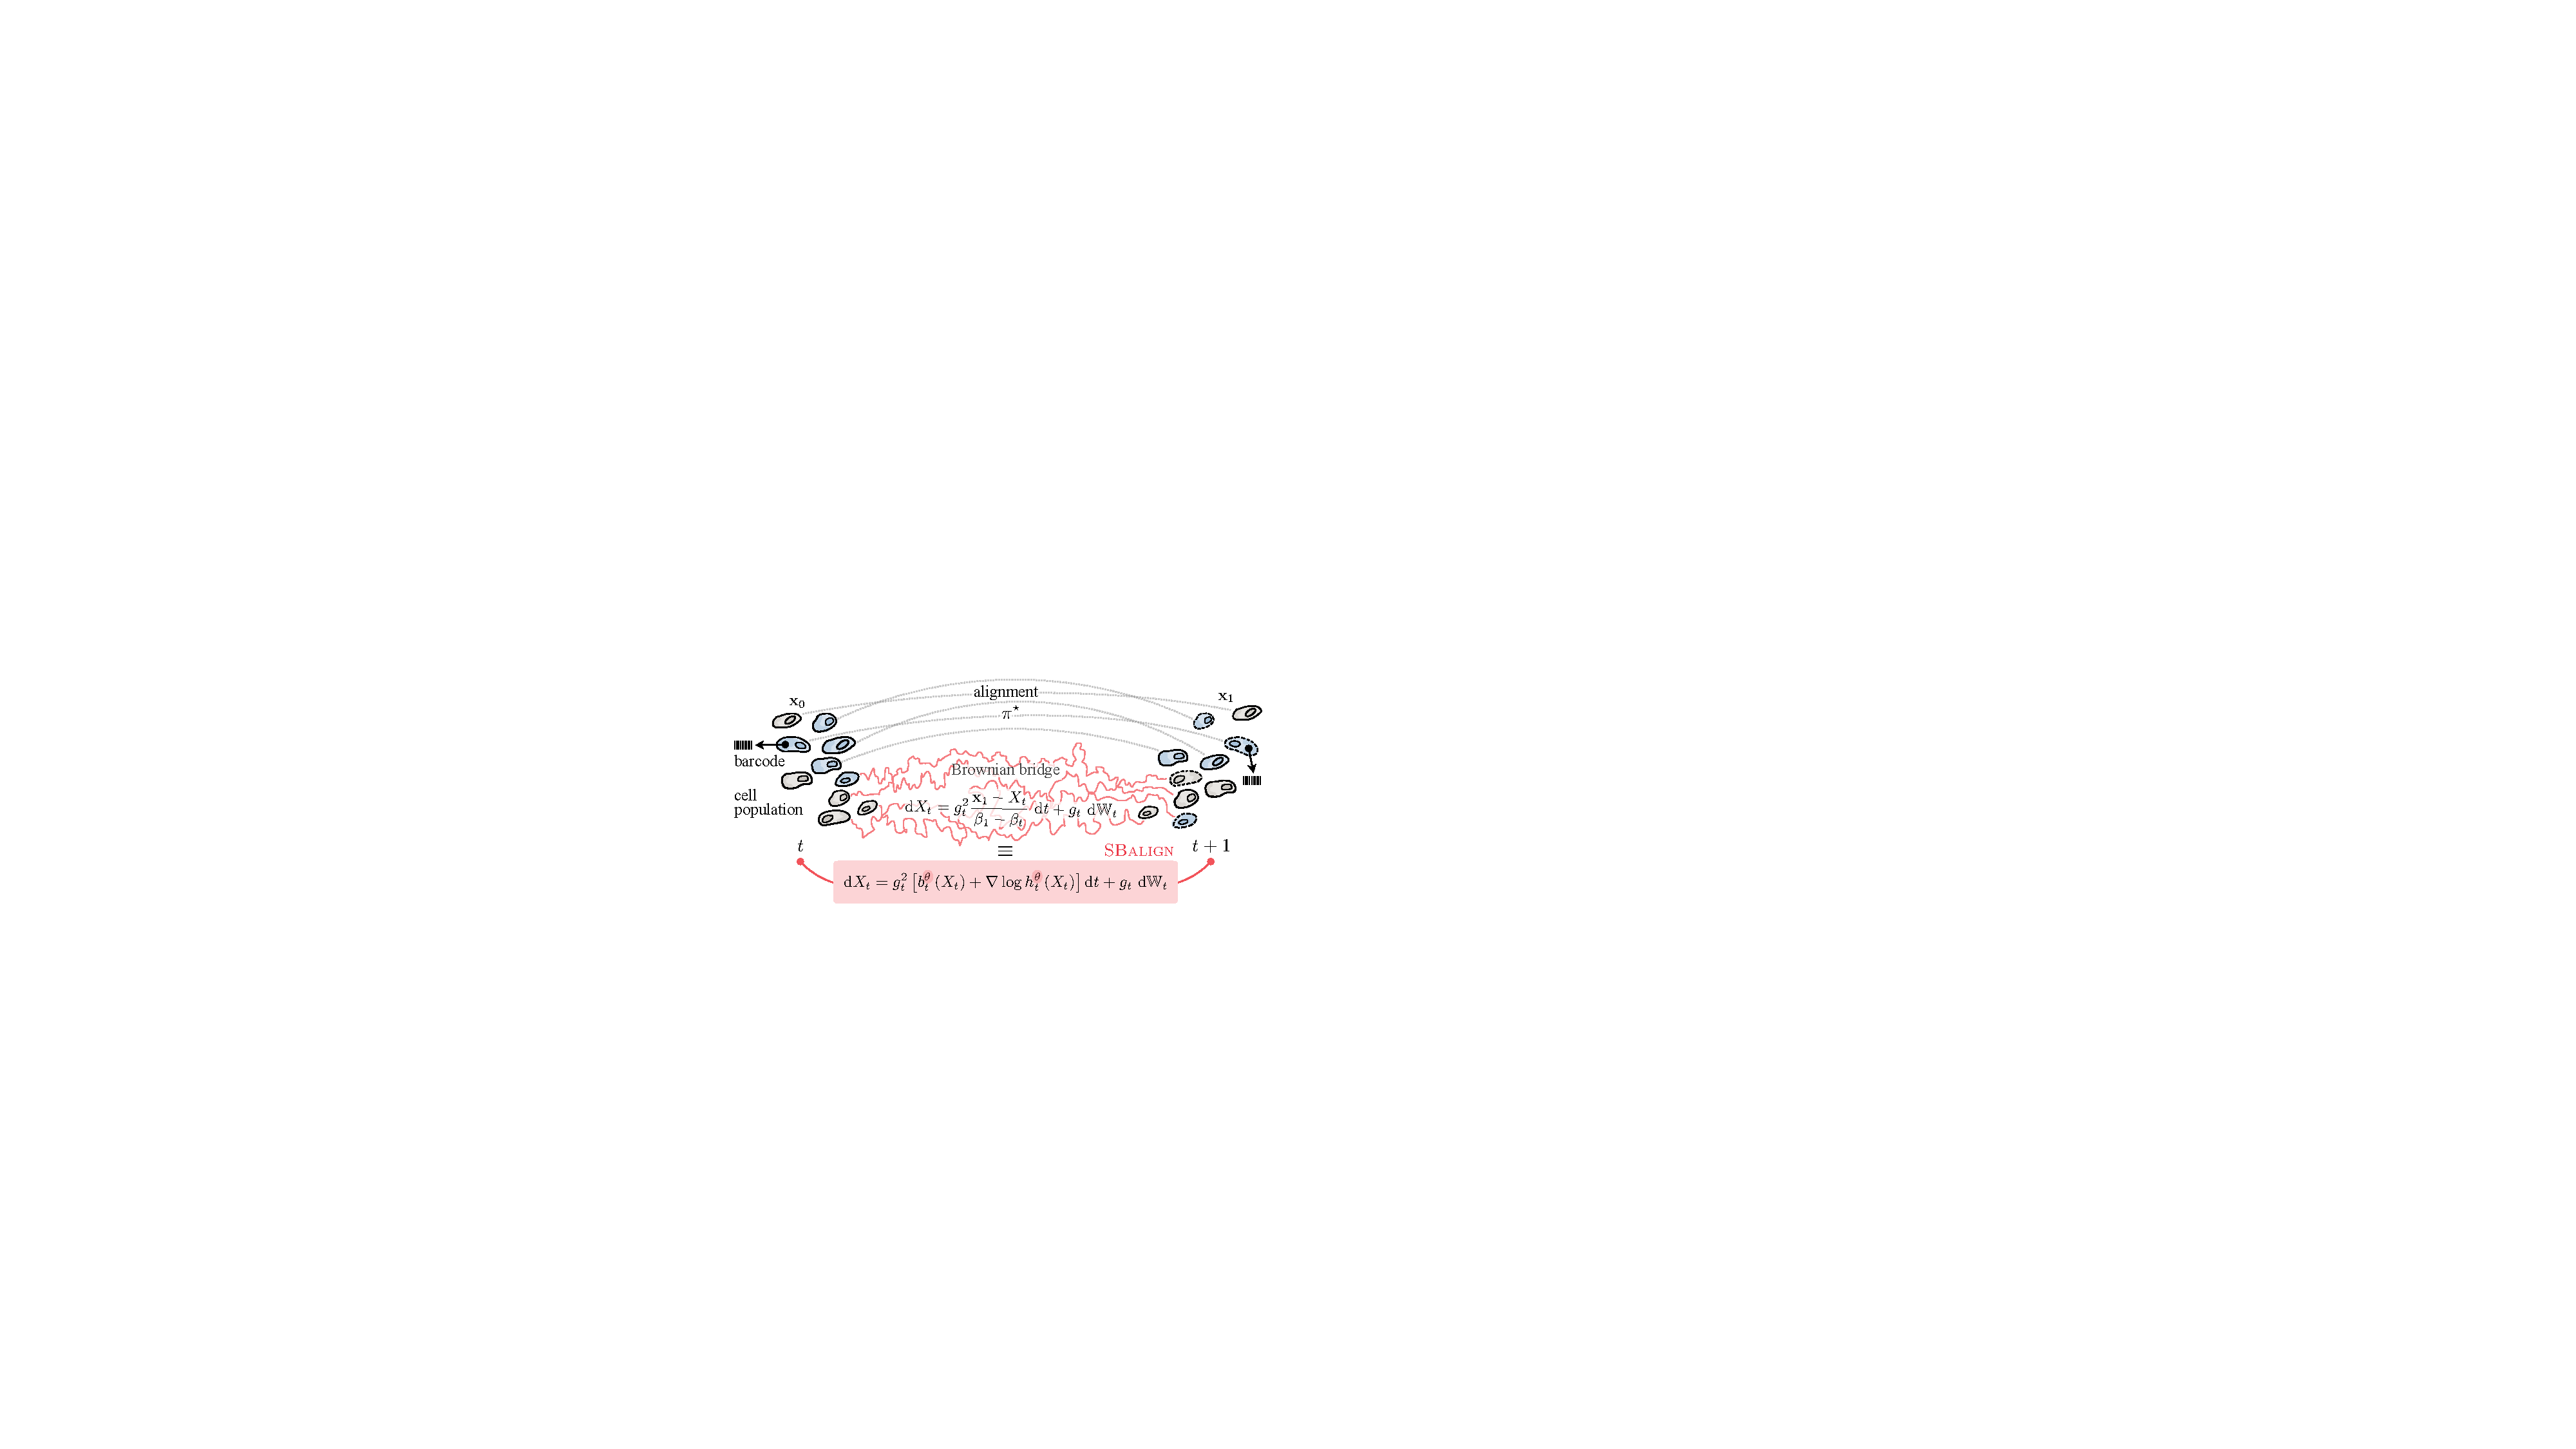
\includegraphics[width=.8\linewidth]{figures/fig_overview_sbalign.pdf}
    \caption{Overview of \textsc{SBalign}: In biological tasks such as protein docking, one is naturally provided with {\em aligned} data in the form of unbound and bound structures of participating proteins. Our goal is to therefore recover a stochastic trajectory from $\x_0$ to $\x_1$. To achieve this, we connect the characterization of an SDE conditioned on $\x_0$ and $\x_1$ (utilizing the Doob's \emph{$h$-transform}) with that of a Brownian bridge between $\x_0$ and $\x_1$ (classical Schr\"odinger bridge theory). We show that this leads to a simpler training procedure with lower variance and strong empirical results.}
    \label{fig:overview_proteins}
\end{figure}

Despite the wide success, a significant limitation of existing frameworks for solving \acrshortpl{DSB} is that they fail to capture the \emph{alignment} of data: If $\distinit, \distend$ are two (empirical) distributions between which we wish to interpolate, then a tacit assumption in the literature is that the dependence of $\distinit$ and $\distend$ is unknown and somehow has to be recovered. Such an assumption, however, ignores important scenarios where the data is \emph{aligned}, meaning that the samples from $\distinit$ and $\distend$ naturally come in pairs $(\x^i_0,\x^i_1)_i^{N}$, which is common in many biological phenomena. Proteins, for instance, undergo conformational changes upon interactions with other biomolecules (protein docking, see Fig.~\ref{fig:overview_proteins}). The goal is to model conformational changes by recovering a (stochastic) trajectory $\x_t$ based on the positions observed at two-time points $\left(\x_0, \x_1\right)$. Failing to incorporate this alignment would mean that we completely ignore information on the correspondence between the initial and final points of the molecules, resulting in a much harder problem than necessary.
Beyond, the recent use of SBs has been motivated by an important task in molecular biology: Cells change their molecular profile throughout developmental processes \citep{schiebinger2019optimal,bunne2022proximal} or in response to perturbations such as cancer drugs \citep{lotfollahi2019scgen,bunne2021learning}. As most measurement technologies are destructive assays, i.e., the same cell cannot be observed twice nor fully profiled over time, these methods aim at reconstructing cell dynamics from \emph{unpaired} snapshots.
Recent developments in molecular biology, however, aim at overcoming this technological limitation. For example, \citet{chen2022live} propose a transcriptome profiling approach that preserves cell viability. \citet{weinreb2020lineage} capture cell differentiation processes by clonally connecting cells and their progenitors through barcodes (see illustrative Figure in Supplement).

\looseness -1 Motivated by these observations, the goal of this paper is to propose a novel algorithmic framework for solving \acrshortpl{DSB} with (partially) \emph{aligned} data. Our approach is in stark contrast to existing works which, due to the lack of data alignment, all rely on some variants of \acrshort{IPF} \citep{fortet1940resolution, kullback1968probability} and are thus prone to numerical instability. On the other hand, via a combination of the original theory of Schr\"odinger bridges \citep{schrodinger1931umkehrung,leonard2013survey} and the key notion of Doob's \emph{$h$-transform} \citep{doob1984classical, rogers2000diffusions}, we design a novel loss function that completely bypasses the \acrshort{IPF} procedure and can be trained with much lower variance.


To summarize, we make the following contributions:
\begin{itemize}[topsep=0pt]
\item To our best knowledge, we consider, for the first time, the problem of interpolation with \emph{aligned} data. We rigorously formulate the problem in the \acrshort{DSB} framework.

\item Based on the theory of Schr\"odinger bridges and $h$-transform, we derive a new loss function that, unlike prior work on \acrshortpl{DSB}, does not require an \acrshort{IPF}-like procedure to train. We also propose principled regularization schemes to further stabilize training.

\item We describe how interpolating aligned data can provide better reference processes for use in classical \acrshortpl{DSB}, paving the way to hybrid aligned/non-aligned \acrshortpl{SB}.

\item \looseness -1 We evaluate our proposed framework on both synthetic and real data. For experiments utilizing real data, we consider two tasks where such aligned data is naturally available. The first is the task of developmental processes in single-cell biology, and the second is ({\em rigid}) protein docking, where the goal is to predict the 3D structure of the bound complex formed by two proteins, given their unbound 3D structures. Our method demonstrates a considerable improvement over prior methods across various metrics, thereby substantiating the importance of taking the data alignment into account. 

\end{itemize}

\paragraph{Related work.}

Solving \acrshortpl{DSB} is a subject of significant interest in recent years and has flourished in a number of different algorithms \citep{de2021diffusion,chen2021likelihood,vargas2021solving,bunne2022recovering,liu2022deep}. However, all these previous approaches focus on  \emph{unaligned} data, and therefore the methodologies all rely on \acrshort{IPF} and are hence drastically different from ours. In the experiments, we will demonstrate the importance of taking the alignment of data into consideration by comparing our method to these baselines.

An important ingredient in our theory is Doob's $h$-transform, which has recently also been utilized by \cite{liu2023learning} to solve the problem of constrained diffusion. However, their fundamental motivation is different from ours. \cite{liu2023learning} focus on learning the drift of the diffusion model and the $h$-transform \emph{together}, whereas ours is to read off the drift \emph{from} the $h$-transform with the help of {\em aligned data}. Consequently, there is no overlap between the two algorithms and their intended applications. 

To the best of our knowledge, the concurrent work of \citet{tong2023conditional} is the only existing framework that can tackle aligned data, which, however, is not their original motivation. In the context of solving \acrshortpl{DSB}, their algorithm can be seen as learning a vector field that generates the correct \emph{marginal} probability \citep[cf.][Proposition 4.3]{tong2023conditional}. Importantly, this is different from our aim of finding the \emph{pathwise} optimal solution of \acrshortpl{DSB}: If $(\x^i_{0,\textup{test}})_{i=1}^m$ is a test data set for which we wish to predict their destinations, then the framework of \citet{tong2023conditional} can only ensure that the marginal distribution $(\x^i_{1,\textup{test}})_{i=1}^m$ is correct, whereas ours is capable of predicting that $\x^i_{1,\textup{test}}$ is precisely the destination of $\x^i_{0,\textup{test}}$ for each $i$. This latter property is highly desirable in tasks like ML-accelerated protein docking.

\paragraph{Problem formulation.}

Suppose that we are given access to i.i.d. \emph{aligned} data $(\x_0^i,\x_1^i)_{i=1}^N$, where the marginal distribution of $\x^i_0$'s is $\distinit$ and of $\x_1^i$'s is $\distend$. Typically, we view $\distinit$ as the empirical marginal distribution of a stochastic process observed at time $t= 0$, and likewise $\distend$ the empirical marginal observed at $t=\horizon$. The goal is to reconstruct the stochastic process $\Pmargin$ based on $(\x_0^i,\x_1^i)_{i=1}^N$, i.e., to \emph{interpolate} between $\distinit$ and $\distend$.

Such a task is ubiquitous in biological applications. For instance, understanding how proteins dock to other biomolecules is of significant interest in biology and has become a topic of intense study in recent years \citep{ganea2022independent, tsaban2022harnessing, corso2022diffdock}. In the protein docking task, $\x_0^i$ represents the 3D structures of the unbound proteins, while $\x_1^i$ represents the 3D structure of the bound complex. Reconstructing a stochastic process that diffuses $\x_0^i$'s to $\x_1^i$'s is tantamount to recovering the energy landscape governing the docking process.  Similarly, in molecular dynamics simulations, we have access to trajectories $\left(\x_t^i\right)_{t \in [0, 1]}$, where $\x_0^i$ and $\x_1^i$ represent the initial and final positions of the $i$-th molecule respectively. Any learning algorithm using these simulations should be able to respect the provided alignment. 


% \paragraph{Diffusion Schr\"odinger bridges.}

% To solve the interpolation problem, in \cref{sec:Methods}, we will invoke the framework of \acrshortpl{DSB}, which are designed to solve interpolation problems with \emph{unaligned} data. More specifically, given two marginals $\distinit$ and $\distend$, the \acrshort{DSB} framework proceeds by first choosing a reference process $\refpro$ using prior knowledge, for instance a simple Brownian motion, and then solve the entropy-minimization problem over all stochastic processes $\Pmargin$:
% \begin{equation}
% \label{eq:SB}
% \tag{SB}
% \min_{ \substack{ \Pinit = \distinit, \; \Pend = \distend} } \KL(\Pmargin \| \refpro).
% \end{equation}
%
% Despite the fact that many methods exist for solving \eqref{eq:SB}  \citep{de2021diffusion,chen2021likelihood,vargas2021solving,bunne2022recovering}, none of these approaches are capable of incorporating \emph{alignment} of the data. This can be seen by inspecting the objective \eqref{eq:SB}, in which the coupling information $(\x_0^i,\x_1^i)$ is completely lost as only its individual marginals $\distinit,\distend$ play a role therein. Unfortunately, it is well-known that tackling the marginals separately necessitates a forward-backward learning process known as the \acrlong{IPF} procedure \citep{fortet1940resolution,kullback1968probability}, which constitutes the primary reason of high variance training, thereby confronting \acrshortpl{DSB} with numerical and scalability issues. Our major contribution, detailed in the next section, is therefore to devise the first algorithmic framework that solves the interpolation problem with aligned data \emph{without} resorting to IPF.

% TODO: Update this section with camera-ready version of the paper.

\subsection{\textsc{SBalign}: Aligned Diffusion Schr\"odinger Bridges}

In this section, we derive a novel loss function for \acrshortpl{DSB} with aligned data by combining two classical notions: The theory of \acrlongpl{SB} \citep{schrodinger1931umkehrung,leonard2013survey,chen2021stochastic} and Doob's $h$-transform \citep{doob1984classical, rogers2000diffusions}. We then describe how solutions to DSBs with aligned data can be leveraged in the context of classical \acrshortpl{DSB}.

\paragraph{Static SB and aligned data.}

Our starting point is the simple and classical observation that \eqref{eq:SB} is the continuous-time analogue of the \emph{entropic optimal transport}, also known as the \emph{static} \acrlong{SB} problem \citep{leonard2013survey,chen2021stochastic,peyre2019computational}:
\begin{equation}
\label{eq:static-SB}
\Pssol \defeq \argmin_{ \substack{ \Pinit = \distinit, \; \Pend = \distend} } \KL( \mathbb{P}_{0,1} \| \refprobase_{0,1}),
\end{equation}
where the minimization is over all \emph{couplings} of $\distinit$ and $\distend$, and $\refprobase_{0,1}$ is simply the joint distribution of $\refpro$ at $t=0,\horizon$. In other words, if we denote by $\Psol$ the stochastic process that minimizes \eqref{eq:SB}, then the joint distribution $\Psol[0,\horizon]$ necessarily coincides with the $\Pssol$ in \eqref{eq:static-SB}. Moreover, since in \acrshortpl{DSB}, the data is always assumed to arise from $\Psol$, we see that:
\begin{quote}
The \emph{aligned} data $(\x_0^i,\x_1^i)_{i=1}^N$ constitutes samples of $\Pssol$.
\end{quote}
This simple but crucial observation lies at the heart of all derivations to come. 

Our central idea is to represent $\Psol$ via two different, but equivalent, characterizations, both of which involve $\Pssol$: That of a \emph{mixture} of reference processes with pinned end points, and that of conditional \acrlongpl{SDE}.



\paragraph{$\Psol$ from $\Pssol$: $\refpro$ with pinned end points.}

For illustration purposes, from now on, we will assume that the reference process $\refpro$ is a Brownian motion with diffusion coefficient $\volat$:
% \footnote{\looseness -1 Extension to more involved reference processes is conceptually straightforward but notationally clumsy. Furthermore, reference processes of the form \eqref{eq:gtWt} are dominant in practical applications \citep{song2020score, bunne2022recovering}, so we omit the general case. }
\begin{equation}
\label{eq:gtWt}
\dd \refpro = \volat \dWiener.
\end{equation}
In this case, it is well-known that $\refpro$ \emph{conditioned} to start at $\x_0$ and end at $\x_1$ can be written in another \acrshort{SDE} \citep{mansuy2008aspects, liu2023learning}:
\begin{equation}
\label{eq:BB}
\dd X_t = \volatsq[\ctime] \frac{\x_1-X_t}{\cvolat[\horizon]-\cvolat[\ctime]} \dt + \volat\dWiener
\end{equation}
where $X_0 = \x_0$ and %, $\dWiener$ is itself a Brownian motion, and 
\begin{equation}
\cvolat\defeq \int_0^\ctime \volatsq \dd s.
\end{equation}We call the processes in \eqref{eq:BB} the \emph{scaled Brownian bridges} as they generalize the classical Brownian bridge, which corresponds to the case of $\volat \equiv 1$.

The first characterization of $\Psol$ is then an immediate consequence the following classical result in \acrlong{SB} theory: Draw a sample $(\x_0, \x_1) \sim \Pssol$ and connect them via \eqref{eq:BB}. The resulting path is a sample from $\Psol$ \citep{leonard2013survey, chen2021stochastic}. In other words, $\Psol$ is a \emph{mixture} of scaled Brownian bridges, with the mixing weight given by $\Pssol$.


\paragraph{$\Psol$ from $\Pssol$: SDE representation.}



Another characterization of $\Psol$ is that it is itself given by an \acrshort{SDE} of the form \citep{leonard2013survey, chen2021stochastic}
\begin{equation}
\label{eq:SB-SDE}
\dd X_t = \volatsq[\ctime]\fdrift(X_t) \dt + \volat\dWiener.
\end{equation}
Here, $\fdrift: \R^d \to \R^d$ is a time-dependent drift function that we wish to learn.


Now, by Doob's h-transform, we know that the \acrshort{SDE} \eqref{eq:SB-SDE} \emph{conditioned} to start at $\x_0$ and end at $\x_1$ is given by another \acrshort{SDE}  \citep{doob1984classical,rogers2000diffusions}:
\begin{equation}
\label{eq:SB-SD-conditioned}
\dd X_t = \volatsq[\ctime]\bracks*{\fdrift(X_t) + \nabla \log \doob(X_t) }\dt +\volat \dWiener
\end{equation}
where $\doob(\x) \defeq \prob(X_1 = \x_1\vert X_t = \x)$ is the \emph{Doob's $h$ function}. Notice that we have suppressed the dependence of $\doob$ on $\x_0$ and $\x_1$ for notational simplicity. % \footnote{The fact $\doob$ does not depend on the starting point $\x_0$ is easily understood: An \acrshort{SDE} remains the same no matter where it starts.}



\paragraph{Loss function.}

Since both \eqref{eq:BB} and \eqref{eq:SB-SD-conditioned} represent $\Psol$, the solution of the \acrshortpl{DSB}, the two \acrshortpl{SDE} must coincide. 
% This in turn implies that, for all $(\x_0,\x_1)\sim\Pssol$, we must have
% \begin{equation}
% \fdrift(X_t) + \nabla \log \doob(X_t) =  \frac{\x_1-X_t}{\cvolat[\horizon]-\cvolat[\ctime]}.
% \end{equation}
~In other words, suppose we parametrize $\fdrift$ as $\fdrift^\theta$, then, by matching terms in \eqref{eq:BB} and \eqref{eq:SB-SD-conditioned}, we can learn the optimal parameter $\theta^\star$ via optimization of the loss function
\begin{equation}
\label{eq:loss}
\Loss(\theta) \defeq \exof*{\int_0^1 \norm*{ \frac{\x_1-X_t}{\cvolat[\horizon]-\cvolat[\ctime]}-\nabla \log \doob^\theta(X_t)}^2 \dt  }
\end{equation}where $\doob^\theta$ is determined by $\fdrift^\theta$ as well as the drawn samples $(\x_0,\x_1)$. In short, assuming that, for each $\theta$, we can compute $\doob^\theta$ \emph{based only on} $\fdrift^\theta$, we can then backprop through \eqref{eq:loss} and optimize it using any off-the-shelf algorithm.


\paragraph{A slightly modified \eqref{eq:loss}.}
Even with infinite data and a neural network with sufficient capacity, the loss function defined in \eqref{eq:loss} does converge to 0. For the purpose of numerical stability, we instead propose to modify \eqref{eq:loss} to:
\begin{equation}
\label{eq:loss_modified}
\Loss(\theta) \defeq \exof*{\int_0^1 \norm*{\frac{\x_1-X_t}{\cvolat[\horizon]-\cvolat[\ctime]}- \left(\fdrift^\theta + \nabla \log \doob^\theta(X_t)\right)}^2 \dt  }
\end{equation}which is clearly equivalent to \eqref{eq:loss} at the true solution of $\fdrift$. Notice that \eqref{eq:loss_modified} bears a similar form as the popular score-matching objective employed in previous works \citep{song2019generative,song2020score}:
\begin{equation}
\label{eq:score_matching}
\Loss(\theta) \defeq \exof*{\int_0^1 \norm*{\nabla \log p(\x_t | \x_0)- s^\theta(X_t, t)}^2 \dt  },
\end{equation}
where the term $\frac{\x_1-X_t}{\cvolat[\horizon]-\cvolat[\ctime]}$ is akin to $\nabla \log p(\x_t | \x_0)$, while $\left(\fdrift^\theta + \nabla \log \doob^\theta(X_t)\right)$ corresponds to $s^\theta(X_t, t)$. 

 \begin{algorithm}[t]
   \caption{\textsc{SBalign}}
   \label{alg:SBalign}
\begin{algorithmic}
   \STATE {\bfseries Input:} Aligned data $(\x^i_0,\x^i_1)_{i=1}^N$, learning rates $\lrf,\lrb$, training iterations $K$. %\dots  data $x_i$, size $m$
   \STATE {\bfseries Output:} Optimal drift $\fdrift^\theta$ and parameterization $m^{\phi}$ of the "softened" Doob's $h$-transform $\doobs$
%   \STATE {\bfseries Construct \eqref{eq:GaussianSB}:} Compute the means and covariances of $\distinit, \distend$.
%   \REPEAT
\smallskip
   \STATE Initialize $\paramf \subs \paramf_0$, $\paramb \subs \paramb_0$
   \FOR{$k=1$ {\bfseries to} $K$} 
   \STATE Draw a mini-batch of samples from $(\x^i_0,\x^i_1)_{i=1}^N$
%   \FOR{$j=1$ {\bfseries to} $\inneriter$}   
%   \IF{$j \mod \caching = 0$}
   \STATE Compute empirical average of loss $\Loss$ \eqref{eq:loss_final} with mini-batch
%   \ENDIF
%   \STATE Compute $\lossb$ via \eqref{eq:loss-backward}
   \STATE Update $\paramb \subs \paramb - \lrb\nabla \Loss(\theta,\phi)$
%   \ENDFOR
%   \FOR{$j=1$ {\bfseries to} $\inneriter$}   
%   \IF{$j \mod \caching = 0$}
%   \STATE Simulate \eqref{eq:GSB-sde-backward} with $\point_\horizon \sim \distend$
%   \ENDIF
%   \STATE Compute $\lossf$ via \eqref{eq:loss-forward}
   \STATE Update $\paramf \subs \paramf - \lrf\nabla \Loss(\theta,\phi)$
   \ENDFOR
%   \ENDFOR
%   \UNTIL{$noChange$ is $true$}
\end{algorithmic}
\end{algorithm}

\paragraph{Computing $\doob^\theta$.}

Inspecting $\doob$ in \eqref{eq:SB-SD-conditioned}, we see that, given $(\x_0,\x_1)$, it can be written as the conditional expectation of an indicator function:
\begin{equation}
\label{eq:h-semigroup}
\doob(\x) = \prob(X_1 = \x_1\vert X_t = \x) = \exof*{
\one_{\{\x_1\}}\vert X_t = \x}
\end{equation}where the expectation is over \eqref{eq:SB-SDE}. Functions of the form \eqref{eq:h-semigroup} lend itself well to computation since it solves simulating the \emph{unconditioned} paths.
% since the Feymann-Kac formula, which offers an representation via simulating the \emph{unconditional} paths and has been well-studied in fields such as physics \cite{}, financial engineering \citep{}, and machine learning \citep{}. 
Furthermore, in order to avoid overfitting on the given samples, it is customary to replace the "hard" constraint $\one_{\{\x_1\}}$ by its \emph{smoothed} version \citep{zhang2021path, holdijk2022path}: 
\begin{equation}
\label{eq:softdoob}
\doobs(\x) \defeq \exof*{  \exp\parens*{-\frac{1}{2\reg}\norm{X_\horizon-\x_1}^2 }  \vert X_t = \x}.
\end{equation}Here, $\reg$ is a regularization parameter that controls how much we ``soften'' the constraint, and we have $\lim_{\reg\to 0} \doobs = \doob$.


Although the computation of \eqref{eq:softdoob} can be done via a standard application of the Feynman-Kac formula \citep{rogers2000diffusions}, an altogether easier approach is to parametrize $\doobs$ by a second neural network $m^{\phi}$ and perform alternating minimization steps on $\fdrift^\theta$ and $m^{\phi}$. This way, we can also avoid simulating even the unconditional paths of \eqref{eq:SB-SDE}, and thereby further reducing the variance in training.

% To summarize, we have
% Combining the above, we shall adopt the Feymann-Kac formula for computing $\doobs$:
% \begin{align}
% \label{eq:logdoobs}
% &\nabla \log \doobs(\x) \\ 
% \nn
% &\hspace{5mm}=\lim_{\ctimealt \searrow \ctime} \frac{\mathbb{E}_{\textup{\eqref{eq:SB-SDE}}} \bracks*{  \exp\parens*{-\frac{1}{2\reg}\norm{X_\horizon-\x_1}^2 } \int_\ctime^{\ctimealt} \volat[s]\dWiener \vert X_t = \x  }  }{(\ctimealt-\ctime) \mathbb{E}_{\textup{\eqref{eq:SB-SDE}}} \bracks*{ \exp\parens*{-\frac{1}{2\reg}\norm{X_\horizon-\x_1}^2 }  \vert X_t = \x} }.
% \end{align}
% The generalization of \eqref{eq:logdoobs} to the case of $\fdrift^\theta$ is straightforward. It remains to neural net everything.

\begin{figure*}[t]
    \centering
    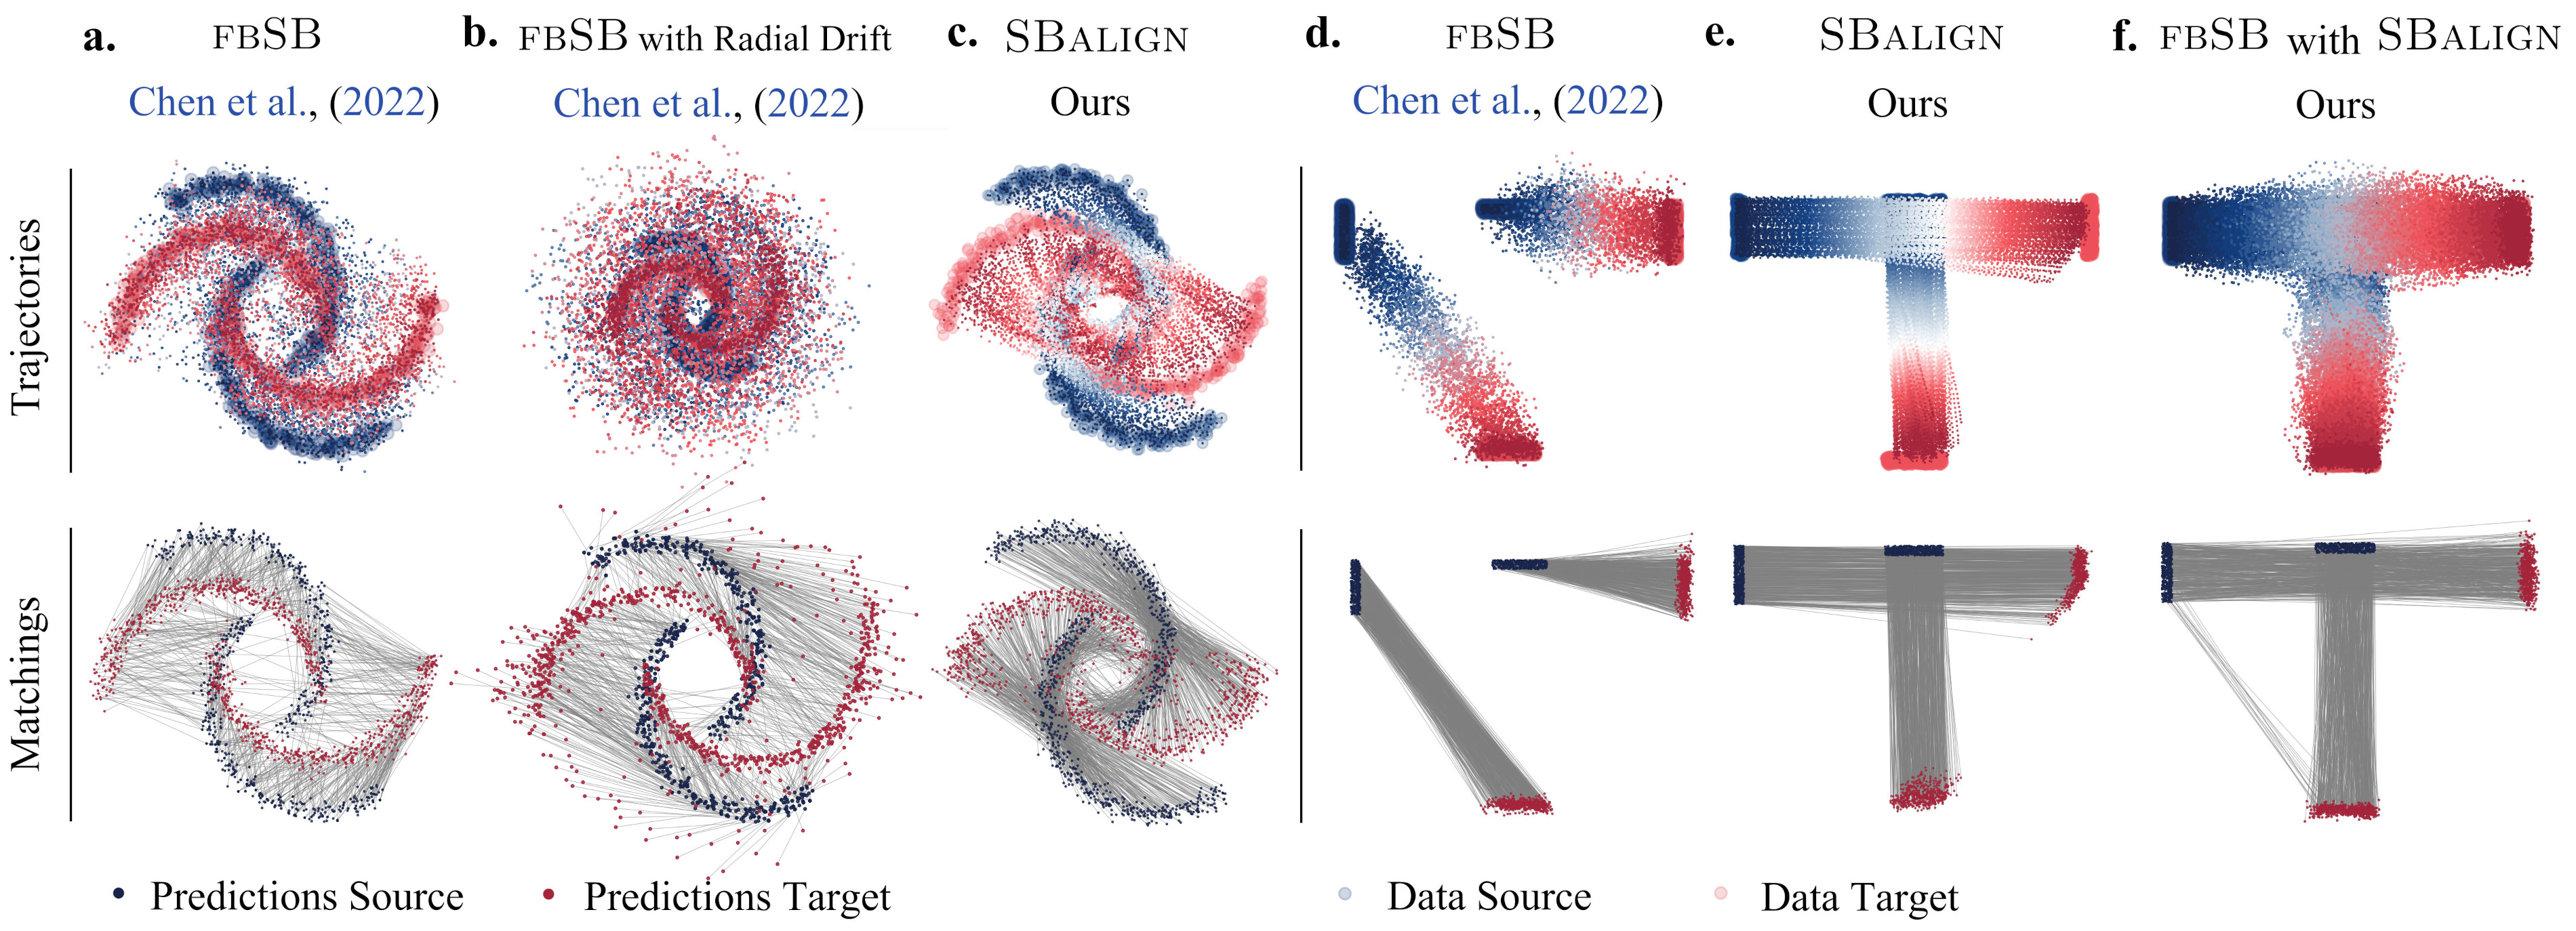
\includegraphics[width=\textwidth]{figures/fig_results_synthetic.jpg}
    \caption{Experimental results on the Moon dataset (\textbf{a-c}) and T-dataset (\textbf{d-f}). The top row shows the trajectory sampled using the learned drift, and the bottom row shows the matching based on the learnt drift. Compared to other baselines, \textsc{SBalign} is able to learn an appropriate drift respecting the true alignment. (\textbf{f}) further showcases the utility of \textsc{SBalign}'s learnt drift as a suitable reference process to improve other training methods.}
    \label{fig:results_spiral}
\end{figure*}

\paragraph{Regularization.}
Since it is well-known that $\nabla \log\doob$ typically explodes when $\ctime\to 1$ \citep{liu2023learning}, it is important to regularize the behavior of $m^{\phi}$ for numerical stability, especially when $\ctime\to 1$. Moreover, in practice, it is desirable to learn a drift $\fdrift^\theta$ that respects the data alignment \emph{in expectation}: If $(\x_0,\x_1)$ is an input pair, then multiple runs of the \acrshort{SDE} \eqref{eq:SB-SDE} starting from $\x_0$ should, on average, produce samples that are in the proximity of $\x_1$. This observation implies that we should search for drifts whose corresponding $h$-transforms are diminishing.

A simple way to simultaneously achieve the above two requirements is to add an $\ell^2$-regularization term, resulting in the loss function:
% \eqref{eq:logdoobs} is computationally expensive to simulate, because of repeated function calls to to $\fdrift^\theta$, and also suffers from high variance especially in the initial stages of training. 
% Note $\nabla \log \doobs(\x_1) = 0$. We replace $\nabla \log \doobs(\x)$ with a neural network $m^{\phi}$ such that $\norm{m^{\phi}(\x_1)}$ is minimized. The final loss function looks like
\begin{align}
\label{eq:loss_final}
\Loss(\theta,\phi) &\defeq \mathbb{E} \Bigg[\int_0^1 \norm*{\frac{\x_1-X_t}{\cvolat[\horizon]-\cvolat[\ctime]}- \left(\fdrift^\theta + m^{\phi}(X_t)\right)}^2
\\ &\hspace{35mm}+ \lambda_t \norm{m^{\phi}(\x_t)}^2 \dt \Bigg]
\nonumber
\end{align}where $\lambda_t$ can either be constant or vary with time. The overall algorithm is depicted in \cref{alg:SBalign}.


\subsection{Aligned Schr\"odinger Bridges as Prior Processes}
\label{subsec:prior_drift}
% Classical SBs are unsuitable in cases where the alignments are known, because they only consider samples from $\distinit$ and $\distend$ and disregard those drawn from the (optimal) coupling $\pi^\star$. However, the reliance of our method on this crucial knowledge is critical to avoid the necessity of IPF-like iterates but may become a limitation when insufficient information on alignments is available. 

% In such a situation, while it is unrealistic to hope for an accurate solution to the aligned SB problem, the interpolation between $\distinit$ and $\distend$ learned by \textsc{SBalign} (\ref{eq:SB-SDE}) can potentially still be leveraged to obtain a better reference process, when solving a classical SB on the same marginals ---i.e. the term $b_t(X_t)$ learned via \textsc{SBalign} can, in fact, be used \textit{as is} to construct a data-informed alternative $\Tilde{\refpro}$ to the standard Brownian motion (\ref{eq:gtWt}).

% Improved reference processes, either using pre-trained or data-informed ones, have been previously considered in the literature. 
% For instance, both \citet{de2021diffusion} and \citet{chen2021likelihood} use a pre-trained reference process for challenging image interpolation tasks. This approach, however, relies on DSBs trained using the classical score-based generative modeling objective between a Gaussian and the data distribution. It therefore pre-trains the reference process on a related ---but different--- process, i.e., the one mapping Gaussian noise to data rather than $\distinit$ to $\distend$.
% An alternative, proposed by \citet{bunne2022recovering}, draws on the closed-form solution of SBs between two Gaussian distributions, which are chosen to approximate $\distinit$ and $\distend$, respectively.
% Unlike our method, these alternatives construct better prior drifts by falling back to simpler and related tasks, or approximations of the original problem. We instead propose to shape a coarse-grained description of the drift based on alignments sampled directly from $\mathbb{P}_{0,1}$. 

% TODO: Adjust this section and polish.
Our algorithm finds solutions to SBs on aligned data by relying on samples drawn from the (optimal) coupling $\pi^\star$. This is what differentiates it from classical SBs --which instead only consider samples from $\hat{\mathbb{P}}_0$ and $\hat{\mathbb{P}}_1$-- and plays a critical role in avoiding IPF-like iterates. However, \textsc{SBalign} reliance on samples from $\pi^\star$ may become a limitation, when the available information on alignments is insufficient. 

If the number of pairings is limited,  it is unrealistic to hope for an accurate solution to the aligned SB problem. However, the interpolation between $\hat{\mathbb{P}}_0$ and $\hat{\mathbb{P}}_1$ learned by \textsc{SBalign} can potentially be leveraged as a starting point to obtain a better reference process, which can then be used when solving a classical SB on the same marginals. In other words, the drift $b^\text{aligned}_t(X_t)$ learned through \textsc{SBalign} can be used \textit{as is} to construct a data-informed alternative $\tilde{\mathbb{Q}}$ to the standard Brownian motion, defined by paths:
\[
    \tilde{X}_t = b^\text{aligned}_t(\tilde{X}_t) dt + g_t dW_t
\]
Intuitively, solving a standard SB problem with $\tilde{\mathbb{Q}}$ as reference is beneficial because the (imperfect) coupling of marginals learned by \textsc{SBalign} ($\tilde{\mathbb{Q}}_{01}$) is, in general, closer to the truth than $\mathbb{Q}_{01}$.

Improving reference processes through pre-training or data-dependent initialization has been previously considered in the literature. For instance, both \citet{de2021diffusion} and \citet{chen2021likelihood} use a pre-trained reference process for challenging image interpolation tasks. This approach, however, relies on DSBs trained using the classical score-based generative modeling objective between a Gaussian and the data distribution. It, therefore, pre-trains the reference process on a related --but different-- process, i.e., the one mapping Gaussian noise to data rather than $\hat{\mathbb{P}}_0$ to $\hat{\mathbb{P}}_1$.
An alternative, proposed by \citet{bunne2022recovering} draws on the closed-form solution of SBs between two Gaussian distributions, which are chosen to approximate $\hat{\mathbb{P}}_0$ and $\hat{\mathbb{P}}_1$, respectively.
Unlike our method, these alternatives construct prior drifts by falling back to simpler and related tasks, or approximations of the original problem. We instead propose to shape a coarse-grained description of the drift based on alignments sampled directly from $\pi^\star_{01}$. 


\subsection{Empirical Evaluation}
In this section, we evaluate \textsc{SBalign} in different settings involving 2-dimensional synthetic datasets, the task of reconstructing cellular differentiation processes, as well as predicting the conformation of a protein structure and its ligand formalized as rigid protein docking problem.

\subsubsection{Synthetic Dynamics}
\label{sec:sbalign_synthetic}

\begin{figure*}
    \centering
    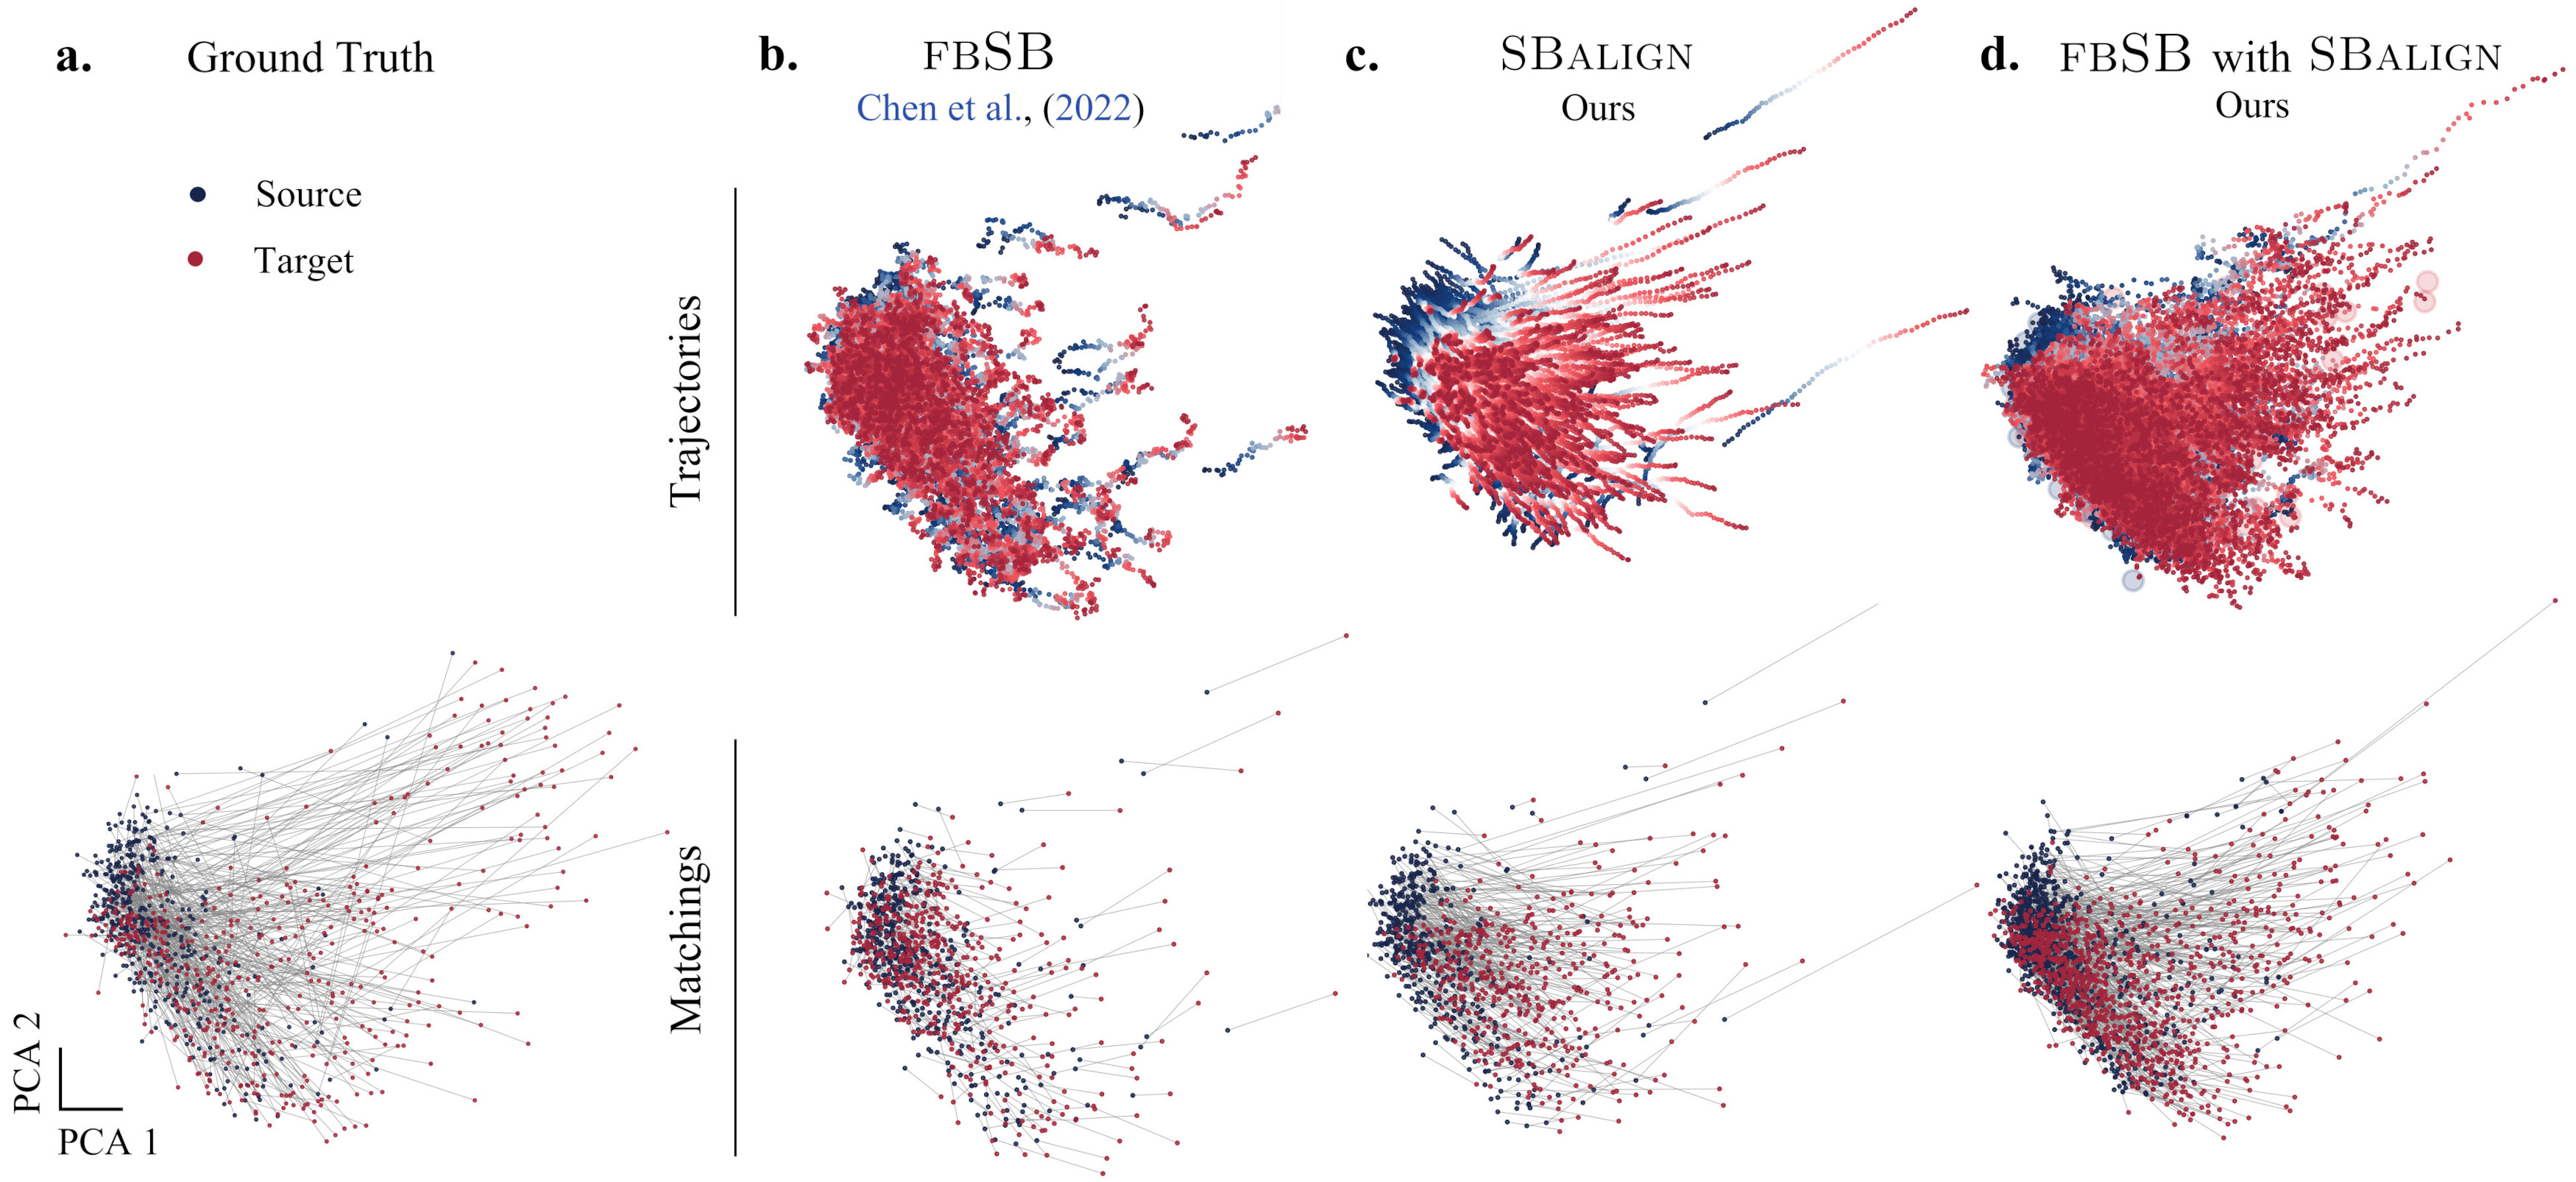
\includegraphics[width=\textwidth]{figures/fig_cell_trajectories_matchings.jpg}
    \caption{Cell differentiation trajectories based on (\textbf{a}) the ground truth and (\textbf{b-d}) learned drifts. \textsc{SBalign} is able to learn an appropriate drift underlying the true differentiation process while respecting the alignment. (\textbf{d}) Using the learned drift from \textsc{SBalign} as a reference process helps improve the drift learned by other training methods.}
    \label{fig:results_cell_traj}
\end{figure*}

We run our algorithm on two synthetic datasets, and compare the results with classic diffusion Schr\"odinger bridge models, i.e., the forward-backward SB formulation proposed by \cite{chen2021likelihood}, herein referred to as \textsc{fbSB}. We equip the baseline with prior knowledge, as elaborated below, to further challenge \textsc{SBalign}.

\paragraph{Moon dataset.}
The first synthetic dataset (Fig.~\ref{fig:results_spiral}a-c) consists of two distributions, each supported on two semi-circles ($\distinit$ drawn in \textit{blue} and $\distend$ in \textit{red}).
$\distend$ was obtained from $\distinit$ by applying a clockwise rotation around the center, i.e., by making points in the upper blue arm correspond to those in the right red one.
This transformation is clearly not the most likely one under the assumption of Brownian motion of particles and should therefore not be found as the solution of a classical SB problem. 
This is confirmed by \textsc{fbSB} trajectories (Fig.~\ref{fig:results_spiral}a), which tend to map points to their closest neighbor in $\distend$ (e.g., some points in the upper arm of $\distinit$ are brought towards the left rather than towards the right). 
While being a minimizer of \eqref{eq:SB}, such a solution completely disregards our prior knowledge on the alignment of particles, which is instead reliably reproduced by the dynamics learned by \textsc{SBalign} (Fig.~\ref{fig:results_spiral}c).

One way of encoding this additional information on the nature of the process is to modify $\refpro$ by introducing a clockwise radial drift, which describes the prior tangential velocity of particles moving circularly around the center.
Solving the classical SB with this updated reference process indeed generates trajectories that respect most alignments (Fig.~\ref{fig:results_spiral}b), but requires a hand-crafted expression of the drift that is only possible in very simple cases.

\paragraph{T dataset.}
In most real-world applications, it is very difficult to define an appropriate reference process $\refpro$, which respects the known alignment without excessively distorting the trajectories from a solution to \eqref{eq:SB}. This is already visible in simple examples like (Fig.~\ref{fig:results_spiral}d-f), in which the value of good candidate prior drifts at a specific location needs to vary wildly in time.
In this dataset, $\distinit$ and $\distend$ are both bi-modal distributions, each supported on two of the four extremes of an imaginary T-shaped area.
We target alignments that connect the two arms of the T as well as the top cloud with the bottom one. We succeed in learning them with \textsc{SBalign} (Fig.~\ref{fig:results_spiral}e) but unsurprisingly fail when using the baseline \textsc{fbSB} (Fig.~\ref{fig:results_spiral}d) with a Brownian motion prior.

\looseness -1 In this case, however, attempts at designing a better reference drift for \textsc{fbSB} must take into account the additional constraint that the horizontal and vertical particle trajectories intersect (see Fig.~\ref{fig:results_spiral}e), i.e., they cross the same area at times $t_h$ and $t_v$ (with $t_h > t_v$). This implies that the drift $b_t$, which initially points downwards (when $t < t_v$), should swiftly turn rightwards (for $t > t_h$).
Setting imprecise values for one of $t_h$ and $t_v$ when defining custom reference drifts for classical SBs would hence not lead to the desired result and, worse, would actively disturb the flow of the other particle group.

\looseness -1 As described in \S~\ref{subsec:prior_drift}, in presence of hard-to-capture requirements on the reference drift, the use of \textsc{SBalign} offers a remarkably easy and efficient way of learning a parameterization of it. For instance, when using the drift obtained by \textsc{SBalign} as reference drift for the computation of the SB baseline (\textsc{fbSB}), we find the desired alignments (Fig.~\ref{fig:results_spiral}f).

\begin{figure*}[t]
    \centering
    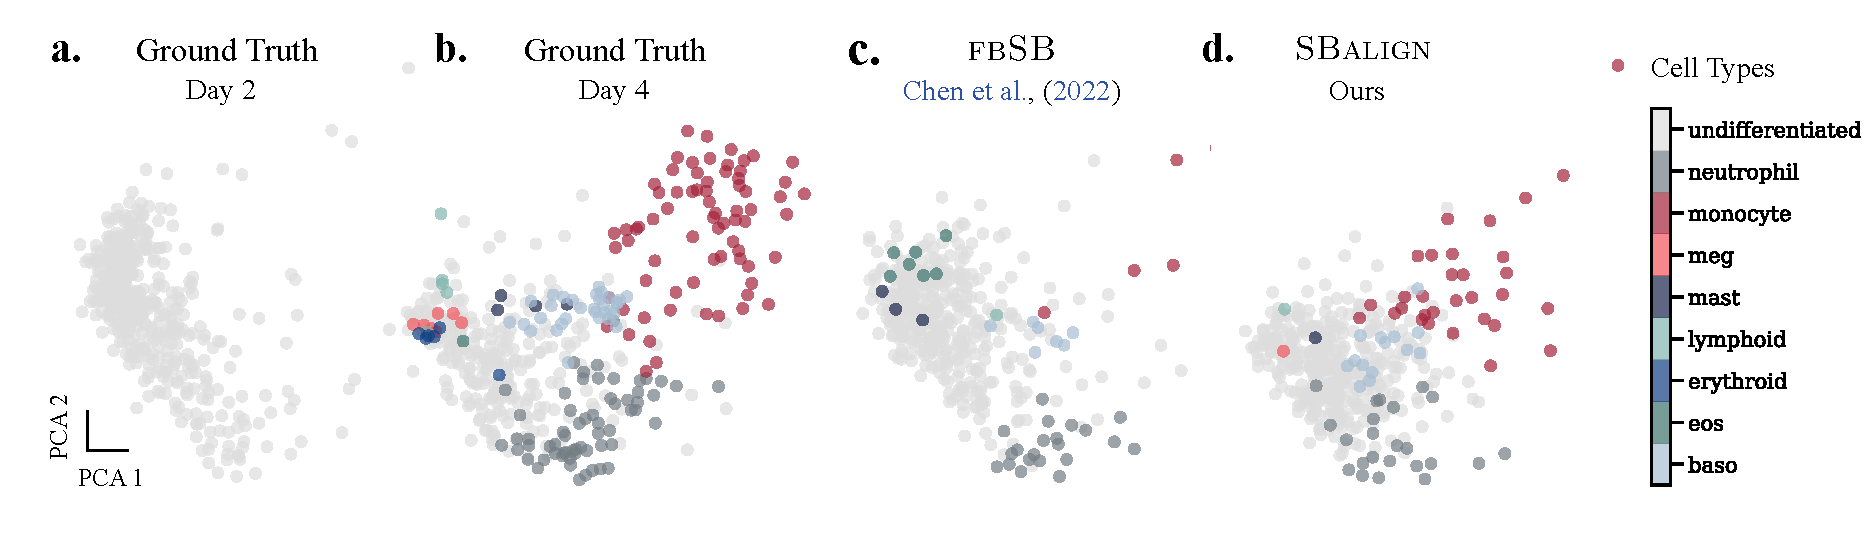
\includegraphics[width=\textwidth]{figures/fig_cell_pred_types.pdf}
    \caption{Cell type prediction on the differentiation dataset. All distributions are plotted on the first two principal components. \textbf{a-b:} Ground truth cell types on day 2 and day 4 respectively. \textbf{c-d:} \textsc{fbSB} and \textsc{SBalign} cell type predictions on day 4. \textsc{SBalign} is able to better model the underlying differentiation processes and capture the diversity in cell types.}
    \label{fig:results_cell_class}
\end{figure*}

\subsubsection{Single-Cell Dynamics}
\label{sec:sbalign_cell}

\looseness -1 Biological processes are determined through heterogeneous responses of single cells to external stimuli, i.e., developmental factors or drugs. Understanding and predicting the dynamics of single cells subject to a stimulus is thus crucial to enhance our understanding of health and disease and the focus of this task.
Most single-cell high-throughput technologies are destructive assays ---i.e., they destroy cells upon measurement--- allowing us to only measure \textit{unaligned} snapshots of the evolving cell population. Recent methods address this limitation by proposing (lower-throughput) technologies that keep cells alive after transcriptome profiling \citep{chen2022live} or that genetically tag cells to obtain a clonal trace upon cell division \citep{weinreb2020lineage}.

To showcase \textsc{SBalign}'s ability to make use of such (partial) alignments when inferring cell differentiation processes, we take advantage of the genetic barcoding system developed by \citet{weinreb2020lineage}. With a focus on fate determination in hematopoiesis, \citet{weinreb2020lineage} use expressed DNA barcodes to clonally trace single-cell transcriptomes over time. The dataset consists of two snapshots: the first, recorded on day 2, when most cells are still undifferentiated (see Fig.~\ref{fig:results_cell_class}a), and a second, on day 4, comprising many different mature cell types (see Fig.~\ref{fig:results_cell_class}b). Using \textsc{SBalign} as well as the baseline \textsc{fsSB}, we attempt to reconstruct cell evolution between day 2 and day 4, all while capturing the heterogeneity of emerging cell types.

\begin{table}
    \caption{\textbf{Cell differentiation prediction results.} Means and standard deviations (in parentheses) of distributional metrics (MMD, $\text{W}_{\epsilon}$), alignment-based metrics ($\ell_2$, RMSD), and cell type classification accuracy.  \vspace{-5pt}}
    \label{tab:results_cells}
     \centering
    \adjustbox{max width=\linewidth}{%
    \begin{tabular}{lccccc}
    \toprule
     & \multicolumn{5}{c}{\textbf{Cell Differentiation}} \\
    \cmidrule(lr){2-6}
    \textbf{Methods} & MMD $\downarrow$ & $\text{W}_\varepsilon \downarrow$ & $\ell_2(\text{PS}) \downarrow$ & RMSD $\downarrow$ & Class. Acc. $\uparrow$ \\
    \midrule
     \textsc{fbSB}& \makecell{1.55e-2\\(0.03e-2)} & \makecell{12.50\\(0.04)} & \makecell{4.08\\(0.04)} & \makecell{9.64e-1\\(0.02e-1)} & \makecell{56.2\%\\(0.7\%)} \\
     \textsc{fbSB} with \textsc{SBalign} & \makecell{5.31e-3\\(0.25e-3)} & \makecell{10.54\\(0.08)} & \makecell{0.99\\(0.12)} & \makecell{9.85e-1\\(0.07e-1)} & \makecell{47.0\%\\(1.5\%)} \\
     \textsc{SBalign} & \makecell{1.07e-2\\(0.01e-2)} & \makecell{11.11\\(0.02)} & \makecell{1.24\\(0.02)} & \makecell{9.21e-1\\(0.01e-1)} & \makecell{56.3\%\\(0.7\%)} \\
     \bottomrule \vspace{-15pt}
    \end{tabular}
}
\end{table}

We benchmark \textsc{SBalign} against previous \acrshortpl{DSB} such as \citep[\textsc{fbSB}]{chen2021likelihood}. Beyond, we compare \textsc{SBalign} in the setting of learning a prior reference process. Naturally, cell division processes and subsequently the propagation of the barcodes are very noisy. While this genetic annotation provides some form of assignment, it does not capture the full developmental process. We thus test \textsc{SBalign} in a setting where it learns a prior from such partial alignments and, plugged into \textsc{fbSB}, is fine-tuned on the full dataset.
To assess the performance of \textsc{SBalign} and the baselines, we monitor several metrics, which include distributional distances, i.e., MMD~\citep{gretton2012kernel} and $\text{W}_{\epsilon}$~\citep{cuturi2013sinkhorn}, as well as average (perturbation scores), i.e., $\ell_2(\text{PS})$, and RMSD. Details on the evaluation metrics can be found in \cref{app:evaluation_metrics}.
Moreover, we also train a simple neural network-based classifier to annotate the cell type on day 4 and we report the accuracy of the predicted vs. actual cell type for all the models.


\textsc{SBalign} finds matching between cell states on days 2 and 4 (Fig.~\ref{fig:results_cell_traj}c, bottom) which resemble the observed ones (Fig.~\ref{fig:results_cell_traj}a) but also reconstructs the entire evolution path of transcriptomic profiles (Fig.~\ref{fig:results_cell_traj}c, top).
It outperforms the baseline \textsc{fbSB} (Table \ref{tab:results_cells}) in all metrics: Remarkably, our method exceeds the performances of the baseline also on distributional metrics and not uniquely on alignment-based ones.
We also leverage \textsc{SBalign} predictions to recover the type of cells at the end of the differentiation process (Fig.~\ref{fig:results_cell_class}d). We do that by training a classifier on differentiated cells observed on day 4, and subsequently classify our predictions. % and applying it to cell statuses predicted by our method.
While capturing the overall differentiation trend, \textsc{SBalign} (as well as \textsc{fbSB}) struggles to isolate rare cell types.
Lastly, we employ \textsc{SBalign} to learn a prior process from noisy alignments based on genetic barcode annotations. When using this reference process within \textsc{fbSB}, we learn an SB which compensates for inaccuracies stemming from the stochastic nature of cell division and barcode redistribution and which achieves better scores on distributional metrics (see Tab.~\ref{tab:results_cells}).

\textsc{SBalign} accurately predicts cellular differentiation processes in hematopoiesis from day 2 to day 4, as visible from the (2D projections of the) learned trajectories and alignments (Fig.~\ref{fig:results_cell_traj}c) and the quantitative evaluation in Table~\ref{tab:results_cells}. \textsc{SBalign} outperforms \textsc{fbSB} in all but the cell-type accuracy metric: Remarkably, our method exceeds the performances of the baseline also on distributional metrics and not uniquely on alignment-based ones. Further, we evaluate how well \textsc{SBalign} recovers the heterogeneity of emerging cell types throughout the developmental process on day 4. The results are displayed in Fig.~\ref{fig:results_cell_class}d and show that, while capturing the overall differentiation trend, \textsc{SBalign} (as well as \textsc{fbSB}) struggles to isolate rare cell types.
Lastly, we employ \textsc{SBalign} to learn a prior process from noisy alignments based on genetic barcode annotations. When using this reference process within \textsc{fbSB}, we learn an SB which compensates for inaccuracies stemming from the stochastic nature of cell division and barcode redistribution and which achieves better scores on distributional metrics (see Tab.~\ref{tab:results_cells}).

\subsection{Discussion}

\vspace{-5pt}
In this paper, we propose a new framework to tackle the interpolation task with aligned data via \acrlongpl{DSB}. Our central contribution is a novel algorithmic framework derived from the Schr\"odinger bridge theory and Doob's $h$-transform. Via a combination of the two notions, we derive novel loss functions which, unlike all prior methods for solving \acrlongpl{DSB}, do not rely on the \acrlong{IPF} procedure and are hence numerically stable. We verify our proposed algorithm on various synthetic and real-world tasks and demonstrate noticeable improvement over the previous state-of-the-art, thereby substantiating the claim that data alignment is a highly relevant feature that warrants further research.

